\documentclass{article}

\usepackage[margin=1.0in]{geometry}
\usepackage{graphicx}
\usepackage{amsmath}
\usepackage{float}
\usepackage{enumitem}

\title{CSC 535 HW3}
\date{9/21/2018}
\author{Simon Swenson}

\begin{document}

\pagenumbering{gobble}
\maketitle
\pagenumbering{arabic}

\large Introduction

\small I completed all of the required homework problems.

\section{Q1}

\subsection{a}

\begin{figure}[!ht]
	\centering
	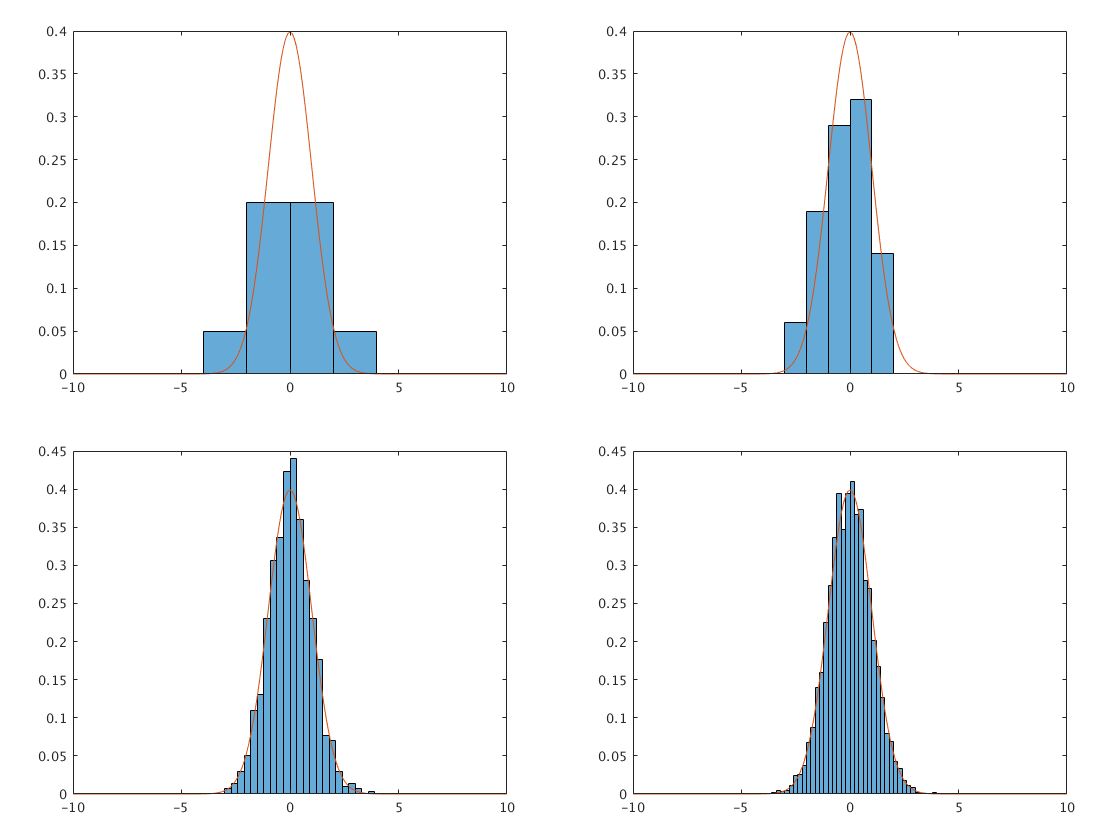
\includegraphics[width=120mm]{q1-all-samples.png}
	\caption{The histograms of various numbers of samples from our sample 
        generator overlayed with the actual PDF ($\mu = 0, \sigma = 1$). 
        Top-left: 10 samples, top-right: 100 samples, bottom-left: 1000 sampes, 
        bottom-right: 10000 samples}
\end{figure}

~\\
~\\
~\\
~\\
~\\
~\\
~\\

\subsection{b}

\begin{figure}[!ht]
	\centering
	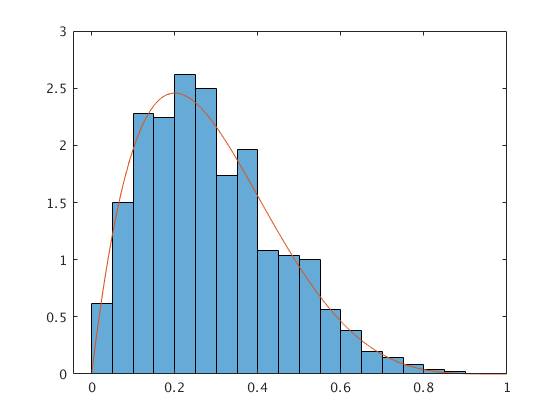
\includegraphics[width=120mm]{q1-beta.png}
	\caption{Using our random sampler to generate samples for the beta 
        distribution, comparing them to ground truth. ($\alpha = 2, \beta = 5$)}.
\end{figure}

~\\
~\\
~\\
~\\
~\\
~\\
~\\
~\\
~\\
~\\
~\\
~\\
~\\
~\\
~\\
~\\
~\\
~\\
~\\
~\\
~\\
~\\
~\\

\section{2}

\subsection{a}

\begin{figure}[!ht]
	\centering
	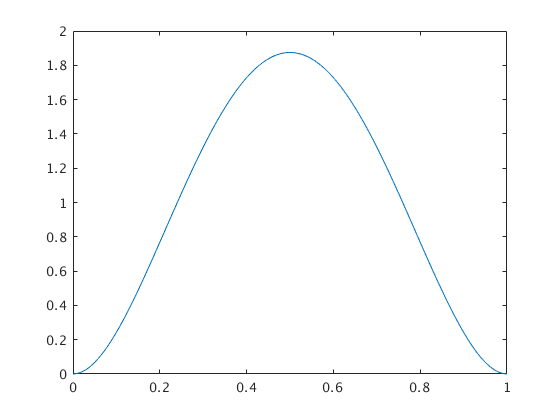
\includegraphics[width=120mm]{q2-prior.png}
	\caption{The given prior, where $\alpha = 3, \beta = 3$. We can interpret 
        this prior as having seen six coin flips, half of which were heads and 
        half of which were tails. After only six coin-flips, we become 
        relatively certain that it is a fair coin: The distribution reaches its 
        peak at 0.5. With lower $\alpha, \beta$ values, the distribution might 
        instead reach its maximum value at 0 and 1, indicating a loaded die 
        with us not having enough information to determine which way the die is 
        loaded. If, instead, our $\alpha, \beta$ values were higher and still 
        equal, the peak at the center would become higher and steeper. This 
        indicates our surity that the coin is fair. Though 
        we are becoming more sure that the coin is fair, the current slope is 
        still not very steep, and we need more coin tosses to verify this. }
\end{figure}

\begin{figure}[!ht]
	\centering
	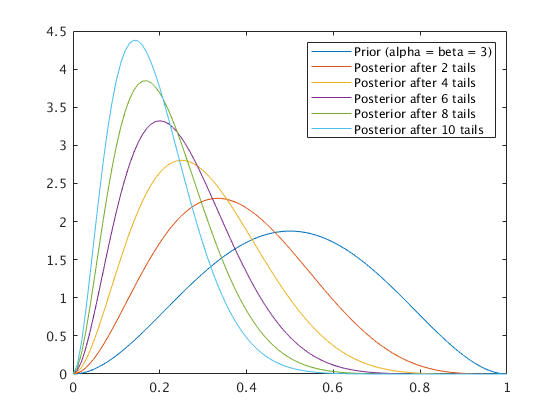
\includegraphics[width=120mm]{q2-all-plots.png}
	\caption{ If, instead of assuming continued fair coin tosses, as was mused 
        upon above, we begin experimenting again and seeing only tails, the 
        distribution quickly shifts away from the center. For each two tails we 
        see with no heads, the peak becomes higher and is shifted further to 
        the left (indicating a bias towards 0, what we interpret as tails) and its 
        slope steeper. With such a heavily biased result, it is no wonder that 
        the PDF changes so quickly. The chances of a fair coin landing tails 
        even six times in a row is very low. }
\end{figure}

~\\
~\\
~\\
~\\
~\\
~\\
~\\
~\\
~\\
~\\
~\\
~\\
~\\
~\\
~\\
~\\
~\\
~\\

\subsection{b}

Recall the PMF for the Poisson distribution:

$$
    p(k | \lambda) = \frac{\lambda^k e^{-\lambda}}{k!}
$$

And the PDF for the Gamma distribution:

$$
    p(x | k, \Theta) = \frac{\beta^{\alpha}}{\Gamma(\alpha)}x^{\alpha - 1} e^{-\beta x}
$$

Then, let's assume that our prior has a Gamma distribution. We then have:

\begin{align*}
    p(\lambda | N) &\propto p(\lambda) p(N | \lambda) \\
        &= p(\lambda) \prod_{n \in N} p(n | \lambda) \\
        &= p(\lambda) \prod_{n \in N} \frac{\lambda^n e^{-\lambda}}{n!} \\
        &= \frac{\beta^{\alpha}}{\Gamma(\alpha)}\lambda^{\alpha - 1} e^{-\beta \lambda} \prod_{n \in N} \frac{\lambda^n e^{-\lambda}}{n!} \\
        &= \beta^{\alpha} \frac{\lambda^{\alpha - 1}e^{-\beta \lambda}}{\Gamma(\alpha)} \prod_{n \in N} \frac{\lambda^n e^{-\lambda}}{\Gamma(n + 1)} \\
\end{align*}

As you can see, the terms line up nicely, showing the conjugacy.

\section{3}

\begin{align*}
    MLE(p(w | X)) &= argmax_w (\prod_{x \in X} p(x | w)) \\
        &\propto argmax_w (log(\prod_{x \in X} p(x | w))) \\
        &= argmax_w (\sum_{x \in X} log(p(x | w))) \\
\end{align*}

At this point, we need to explore the problem further. We are given that the 
distance between the fit polynomial and any given x value follows a Gaussian 
distribution. We can find the mean of this distribution by simply finding the 
y value for the given x value:

$$
\mu = y(x) = w_0 + w_1 x^1 + \dots + w_n x^n
$$

Then, for some unknown variance, the Gaussian distribution is:

$$
p(x | w) = \frac{1}{\sqrt{2 \pi \sigma^2}} e^{-\frac{(y_x - w_0 - w_1 x - \dots - w_n x^n)^2}{2 \sigma^2}}
$$

Note that we use $y_x$ to denote the observed value of x, not the function 
value of x. Substituting this into the equation above, we have:

\begin{align*}
MLE(p(w | X)) &\propto argmax_w (\sum_{x \in X} log(\frac{1}{\sqrt{2 \pi \theta^2}} e^{-\frac{(y_x - w_0 - w_1 x - \dots - w_n x^n)^2}{2 \theta^2}})) \\
    &= argmax_w ( |X| log(\frac{1}{\sqrt{2 \pi \theta^2}}) - \frac{1}{2 \theta^2} \sum_{x \in X} (y_x - w_0 - w_1 x - \dots - w_n x^n)^2) \\
    &\propto argmin_w ( \sum_{x \in X} (y_x - w_0 - w_1 x - \dots - w_n x^n)^2) \\
\end{align*}

This is equivalent to the least squared distance.

~\\
~\\
~\\
~\\
~\\
~\\
~\\
~\\
~\\
~\\
~\\
~\\
~\\
~\\
~\\
~\\
~\\
~\\
~\\
~\\
~\\
~\\
~\\
~\\

\section{4}

\begin{figure}[!ht]
	\centering
	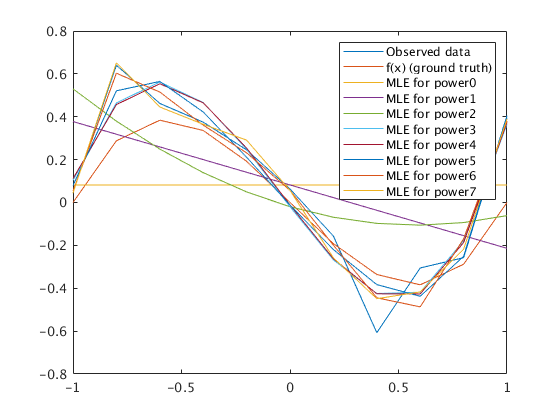
\includegraphics[width=120mm]{q4-mle.png}
	\caption{Using $ (A^T A)^{-1} A^T y $, we find the MLE for the coefficients 
        of the polynomial for various degrees. Ground truth and randomly-generated 
        dataset are present, as well.}
\end{figure}

\begin{figure}[!ht]
	\centering
	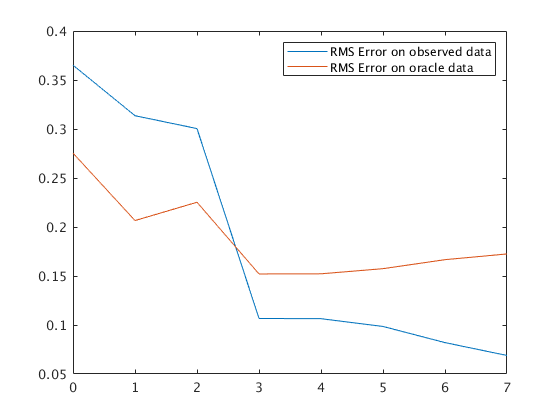
\includegraphics[width=120mm]{q4-rms-error.png}
	\caption{The error of the eight degrees of best-fit polynomials, plotted. 
        You can see a sharp drop at the third degree. This is a good indicator 
        that, in this case, the best degree to pick for the polynomial is three, 
        since gains after that are not as substantial, and the polynomials of 
        higher degree are likely overfitting the data. However, if we take 
        error as our only metric for deciding how good a model is, the 
        polynomial of degree seven wins.
        The \textbf{oracle} provides a different picture from the random sampled 
        data. Using the oracle data to compute error, the error reaches a 
        minimum at exactly degree three. This illustrates the important 
        difference between noisy, real-world data and ideal, oracle data.}
\end{figure}

~\\
~\\
~\\
~\\
~\\
~\\
~\\
~\\
~\\
~\\
~\\
~\\
~\\
~\\
~\\
~\\
~\\
~\\
~\\
~\\
~\\
~\\
~\\
~\\
~\\
~\\
~\\
~\\
~\\
~\\
~\\
~\\
~\\
~\\
~\\
~\\
~\\
~\\
~\\
~\\
~\\
~\\
~\\
~\\
~\\
~\\
~\\
~\\
~\\
~\\
~\\
~\\
~\\
~\\
~\\
~\\

\section{5}

\begin{figure}[!ht]
	\centering
	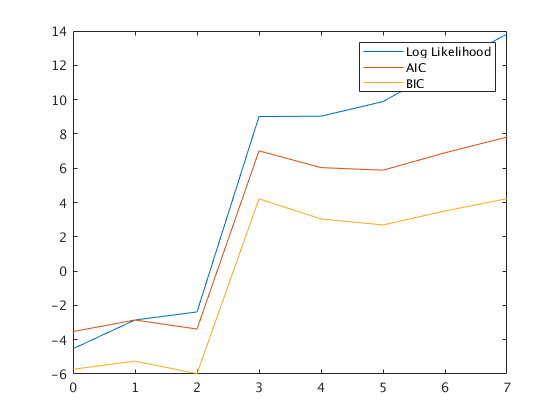
\includegraphics[width=120mm]{q5-eval-metrics.png}
	\caption{\textbf{Log likelihood} for best-fit polynomials of various degrees. Here, 
        we see a clear spike at three, but the value continues steadily 
        increasing. By log likelihood, the suggested best-fit polynomial is the 
        one with the highest degree, seven.
        With \textbf{AIC}, we consider the number of parameters in the model as a 
        penalty. This penalty doing what we wanted by penalizing the 
        higher-order models, but it is simply not doing enough. Eventually, the 
        higher-order polynomials can overpower the metric. Thus, this metric 
        still recommends a polynomial of degree seven.
        Again, \textbf{BIC} is able to succeed in recommending the model with the 
        expected degree, three. The BIC model is very similar to AIC, except 
        that it factors in the number of data points as a penalty as well: If 
        we need too many data points to get a good model, according to BIC, we 
        might have a bad model. As $log(11) > 1$, this model provides a higher 
        penalty than AIC, for our data set. Thus, it is finally able to 
        recommend the desired degree of polynomial: three.}
\end{figure}

~\\
~\\
~\\
~\\
~\\
~\\
~\\
~\\
~\\
~\\
~\\
~\\
~\\
~\\
~\\
~\\

\section{6}

\begin{figure}[!ht]
	\centering
	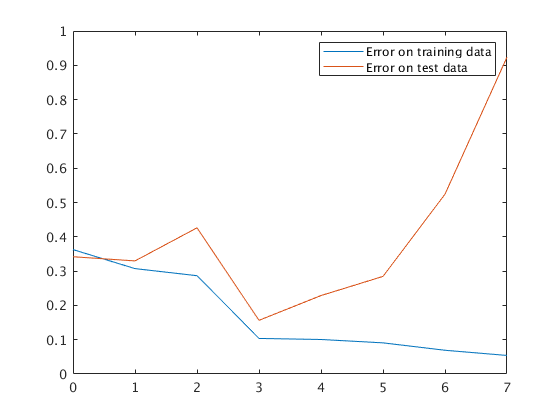
\includegraphics[width=120mm]{q6-rms-err.png}
	\caption{The familiar sudden change at degree three is present for both the 
        training and the test data. However, the difference between the two is 
        that, as the model fits the training data better and better, it 
        actually overfits the data. Thus, while the training error always 
        decreases, the test error starts increasing after three. The training 
        error would recommend degree seven, but the test data, which I would 
        say is more important for providing insight into predictive validity, 
        recommends degree three.}
\end{figure}

\section{7}

\begin{tabular}{r | c}
	Metric & Median Best Polynomial Degree \\
	\hline
	RMS Error on Oracle     & 3 \\
    RMS Error on Observed   & 7 \\
    Log Likelihood          & 7 \\
    AIC                     & 6 \\
    BIC                     & 6 \\
    RMS Error on Train Data & 7 \\
    RMS Error on Test Data  & 3 \\
\end{tabular}

The results of repeated runs are very similar to the results of the trial run
for most metrics. RMS Error on Oracle is the degree we wanted, which makes 
sense, since the error on the oracle data is expected to be high when the model 
has either overfit or underfit. We expect a local minimum at the happy medium 
between the two. Evaluating on oracle data when available can be a decent tool 
for preventing both overfitting and underfitting.

However, when we calculate the RMS error on the observed data, the metric just 
wants more and more coefficients because it has no benchmark and can only 
evaluate on the data it used to fit the model in the first place. This circular 
logic can only lead to a "better" and "better" fit, or in ML terms, overfitting.

Log likelihood has a similar result of a coefficient of seven. As the model 
gets more and more parameters, it can maximize the likelihood better by fitting 
the data points. However, we don't always want to fit the data points perfectly.
Doing so causes overfitting, as in this case.

AIC does slightly better than log likelihood by penalizing models with more 
parameters. However, it still does not perform well enough to suggest the 
preferred polynomial degree (three).

BIC performed the same. While BIC has an additional penalizing term to deal 
with too many data points, the small number of data points in our experiment 
showed that it did little to affect the metric.

An interesting feature of both AIC and BIC is that their best polynomial degree 
differed significantly between runs, varying from two to eight in both cases. 
This is one situation where our single run through the data earlier provided 
a misleading result, that degree three and seven were roughly tied for BIC and 
degree seven barely beating out degree three for AIC.

Dividing the available labeled data into train and test data is the best that 
data scientists can do in certain situations, especially where the data is 
from the real world. However, a key caveat in data science is to \textit{never 
evaluate on your training data}. In order to test if the model can generalize, 
the model should be evaluated on data that it has never seen before. Computing 
the RMS error on the training data is likewise problematic. That explains the 
poor polynomial degree of seven chosen.

Finally the test data provides a robust way to evaluate a model when an oracle 
isn't present. It fulfills a similar role to the oracle, albeit the test data 
is not perfect, just like the training data. However, by evaluating RMS error 
on the test data, we can get a good idea of how well the model generalizes to 
new tasks. In this case, the metric was able to produce the desired polynomial 
degree (three), finding a good balance between overfitting and underfitting, 
just as computing the RMS error on the oracle data had.

\end{document}